\documentclass{article}
\usepackage{tikz}

\usetikzlibrary{positioning}
\usetikzlibrary{arrows}
\usetikzlibrary{arrows.meta}

\tikzset{%
	>={Latex[width=2mm,length=2mm]},
	% Specifications for style of nodes:
	base/.style = {rectangle, rounded corners, draw=black, minimum width=4cm, minimum height=1cm, text centered, font=\sffamily},
	input/.style = {base, fill=blue!30},
	process/.style = {base, fill=red!30},
	output/.style = {base, fill=green!30},
}



\title{Pipeline}
\date{09/02/2018}
\author{Irdi Balla}

\begin{document}
	\maketitle	
	
	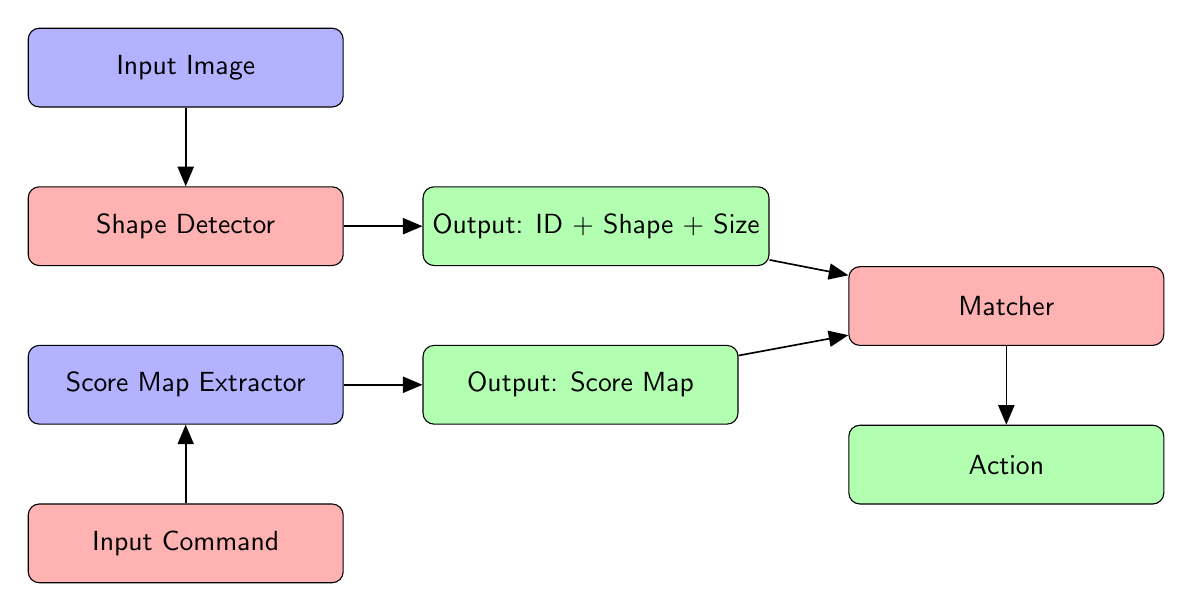
\begin{tikzpicture}[>=triangle 45,font=\sffamily]
		\node (II)[input] {Input Image};
		\node (Shape) [process,below =1cm of II]  {Shape Detector};
		\node (IO) [output,right =1cm of Shape]  {Output: ID + Shape + Size};
		
		\node (ScoreMap) [input,below =1cm of Shape]  {Score Map Extractor};
		\node (IC) [process,below =1cm of ScoreMap]  {Input Command};	
		\node (CO) [output,right =1cm of ScoreMap]  {Output: Score Map};
		
		\node (Matcher) [process, below right=0.0cm and 1cm of IO] {Matcher};
		\node (Action) [output, below = 1cm of Matcher] {Action};
		
		\draw [semithick,->] (II) -- (Shape);
		\draw [semithick,->] (Shape) -- (IO);
		\draw [semithick,->] (IO) -- (Matcher);
		
		\draw [semithick,->] (IC) -- (ScoreMap);
		\draw [semithick,->] (ScoreMap) -- (CO);
		\draw [semithick,->] (CO) -- (Matcher);
		
		\draw [semithick,->] (Matcher) -- (Action);
		
     \end{tikzpicture}
     
     \section{Architecture}
     The Architecture is composed of several parts that pass together to achieve the final Result or as i call it 'Action'.
     \subsection{Environemnt} The environment is a 3D world with different objects that is generated randomly on every test. The environment randomly selects 20 times from the set $\left\{ Cube, Sphere, Pyramid, Cylinder \right\}$ and for each objects it assigns a random size and color. These Objects are placed in the scene in such a way that they dont overlap with each other. The camera represents the robot which looks at this scene from a 45\textsuperscript{o} angle to mimic a situation where the robot is sitting on a table. These objects have to be rearranged to follow the commands.
     \subsection{Shape Detector}
     The Shape Detector is a model trained to recognize the basic shapes from the set $\left\{ , Sphere, Pyramid, Cylinder \right\}$ in an image taken from the environment. This module outputs an ID, a color and a size for the all the shapes that it detects. A bounding region is considered to be a shape if it surpasses a threshold.
     \subsection{Score Map Extractor}\
     The Score Map Extractor is a trained model that takes a command as an input. From the input it extracts the action, the subject on which the action has to happen and the description of the subject. Its ouput is a score map of the geometric cues and semantic segmentation of the words as described by [CITE].
     \subsection{Matcher}
     The matcher has to figure out the best combination of the objects that matches the command. It takes the output of the Shape Detector and Score Map Extractor as its input. The Matcher tries to find the best combination of basic operations [translate, rotate, scale] for every object from the Shape Detector that matches best the Result from the Score Map Extractor. The output from this Module is the 'Action' that is sent to the environment which then performs this action.
	
\end{document}
